\chapter{Discussion}

% Start with the big picture.
Our analysis of the Orion A and Orion B molecular clouds reveals a complex interplay between morphology, topology, and star formation activity. 
By combining perimeter–area scaling, Euler characteristic profiles, and mass–size relations, we obtain a consistent picture of how structural complexity varies across column densities and how these variations relate to the presence of young stellar objects.

% Synthesize the fractal dimension results (global and local).
The global fractal dimension is based on the idea that if a structure is self‑similar—i.e., lacks a characteristic scale—its perimeter and area should follow a power‑law scaling, appearing as a straight line in a log–log diagram.  
Turbulence is known to play a key role in organizing structure within molecular clouds, and the perimeter–area method provides a way to quantify how much this self‑similar behavior influences the observed morphology.

Our global perimeter–area analysis reveals distinct structural regimes within Orion~A, with a clear change in slope that reflects different levels of complexity at low and high column densities.  
In contrast, Orion~B maintains a more uniform fractal signature.  
This contrast already begins to suggest that Orion~A and Orion~B are governed by different physical conditions.

For Orion~A, a double fit is required, indicating a change in the underlying physics. The double fit can be seen in Figure \ref{fig:orion_A_global_double_fit}. 
This transition occurs at a column density of \(N = 1.23 \times 10^{22}\,\mathrm{cm}^{-2}\), marking a physically significant scale.  
At this threshold, the structural properties of Orion~A shift, coinciding with the onset of active star formation and the emergence of dense cores \cite{lada2010star}.  
The concurrent changes in fractal dimension and topology at this scale suggest a direct link between the cloud’s morphology and the physical processes driving star formation.

Without applying the double fit, the global fractal dimension is \(D = 1.35 \pm 0.01\). The single fit for Orion A can be seen in Figure \ref{fig:orion_A_global}. 
This value is in good agreement with previously reported fractal dimensions for molecular clouds derived with alternative methods \cite{elmegreen1996fractal}, where typical values are around \(D \sim 1.3\).  
Numerical simulations based on two‑dimensional compressible turbulence in a self‑gravitating ISM also reproduce similar values \cite{1994fns..book..515Y}.  
Note that many studies report the three‑dimensional fractal dimension, which is related to the two‑dimensional value by adding unity.

When the data are separated into two regimes, we obtain \(D = 1.65 \pm 0.01\) at higher column densities and \(D = 0.97 \pm 0.03\) at lower column densities.  
Although a fractal dimension smaller than 1 is not expected in theory, this result is likely influenced by the limited number of data points contributing to the low‑density fit.  
Even so, the trend is informative: a fractal dimension approaching 1 indicates smoother, simpler boundaries, whereas higher column densities exhibit more complex, space‑filling structures.

Taken together, these results suggest that the processes driving self-similarity—such as turbulence—become less dominant once dense cores emerge.  
Beyond this threshold, the cloud’s structure deviates from scale-free behavior, reflecting the impact of star formation on its morphology.

With methods such as the perimeter–area analysis, it is important to verify that the conclusions drawn are consistent with what is visually apparent in the cloud.  
To this end, Figure~\ref{fig:gallery_global_thresholds_OA} shows Orion~A with three overlaid contours corresponding to low, intermediate, and high column‑density thresholds.  
The intermediate threshold was chosen close to the transition point identified in the global fractal dimension analysis, where the fit was separated into two regimes.

A visual inspection supports the quantitative results.  
At low column densities, Orion~A appears as large, coherent structures with relatively smooth boundaries.  
Around \(N \approx 1.2 \times 10^{22}\,\mathrm{cm}^{-2}\), the morphology begins to change markedly: structures start to fragment, and the cloud breaks up into smaller, more irregular components.  
At even higher column densities, the emission is dominated by compact cores and small-scale features.

This visual progression confirms the double trend inferred from the global analysis.  
Below the transition, the cloud exhibits more complex, interconnected structures, corresponding to the higher global fractal dimension (\(D = 1.65\)).  
Above the transition, the morphology is dominated by simpler, more isolated cores, reflected in the lower fitted fractal dimension (\(D \approx 1\)).  

In Orion~B, by contrast, no such break is required.  
This outcome is broadly consistent with expectations, as Orion~B is known to be a more turbulent molecular cloud.  
In such an environment, scale‑free behavior dominates across the column‑density range analyzed, as reflected in the high quality of the single global fractal dimension fit (Figure \ref{fig:orion_B_global}).  
The emergence of cores does not appear to disrupt the hierarchical structuring.  
Together, these findings provide the first elements of a coherent picture described by the Minkowski functionals.

As with Orion~A, it is important to verify whether the conclusions drawn for Orion~B are consistent with its visual appearance.  
In the corresponding gallery (Figure~\ref{fig:gallery_global_thresholds_OB}), Orion~B breaks down into smaller components relatively quickly, yet the overall visual complexity remains comparable across the examined thresholds.  
The structures appear to fragment in a gradual and continuous manner, with each region breaking into substructures at similar rates.

Because this fragmentation proceeds smoothly across the entire column‑density range, there is no clear transition point that would require separating the perimeter–area relation into distinct regimes.  
The morphology gives the impression of a consistent, scale‑free process, with no abrupt change in structural organization.  

This visual assessment therefore supports the quantitative findings: a single global fractal dimension is sufficient to describe Orion~B, consistent with a more turbulent environment in which fragmentation occurs in a self‑similar way.

It is also instructive to compare these results with measurements obtained for other molecular clouds.  
Studies applying perimeter–area methods or similar techniques have typically found global fractal dimensions in the range \(D \sim 1.2{-}1.4\) for nearby star‑forming regions.  
For example, \cite{falgarone1991hierarchical} reported \(D \approx 1.36\) for CO maps of Perseus and Ophiuchus, while \cite{sanchez2005fractal} found values between 1.25 and 1.35 for a sample of Galactic molecular clouds.  
These values are broadly consistent with the single‑fit results for Orion~A (\(D = 1.35 \pm 0.01\)) and Orion~B (\(D = 1.40 \pm 0.01\)), reinforcing the interpretation that the large‑scale morphology of these clouds is comparable to that of other regions in the Milky Way.

What is less commonly reported, however, is the clear break we observe in Orion~A at \(N = 1.23 \times 10^{22}\,\mathrm{cm}^{-2}\).

Naturally, this method has limitations.  
Numerical errors can arise when calculating perimeters and areas for very small structures at high column densities.  
Straight contours, resulting from limited observational resolution, should also be avoided, as they can distort the scaling relationships on which the method relies.

The local fractal dimension builds on the perimeter–area relation, but in this case the relation is inverted to obtain a proxy for the boundary complexity of individual structures.  
This measure offers a more nuanced view than the global approach, capturing how structural complexity evolves with column density on a local scale.

The local fractal dimension calculated at each column‑density threshold shows a consistent trend toward \(D \approx 2\) at higher thresholds for both Orion~A and Orion~B (Figure \ref{fig:local_Orion_A_B}).  
This behavior appears to arise not from the increasing complexity of individual structures, but rather from the growing, interconnected network of cores, fibers, and filaments that emerge as the cloud fragments at higher column densities.
The average local fractal dimension for both Orion~A and Orion~B is approximately 1.7, which remains within the expected range for molecular clouds. This value suggests that, on average, the boundaries of structures in both regions are moderately complex—more intricate than simple geometric shapes, but not fully space-filling. Such averages are consistent with previous studies and support the interpretation that turbulence and hierarchical fragmentation are key drivers of cloud morphology at these scales.

An intriguing benchmark for interpreting the local fractal dimension comes from the classical theory of turbulence developed by Kolmogorov \cite{kolmogorov1962refinement}.  
In this framework, the energy spectrum of incompressible turbulence follows a power-law scaling of the form \( E(k) \propto k^{-5/3} \), where \( k \) is the wavenumber.  
This spectral slope corresponds to a projected (2D) fractal dimension of approximately \( D \approx 1.7 \), which is often used as a reference point for the morphology of turbulent structures in astrophysical environments.

In molecular clouds, a local fractal dimension approaching this value is commonly interpreted as evidence for Kolmogorov-like turbulent behavior, particularly in low-compression or subsonic regimes.  
In our results, we observe that many of the extracted structures cluster around this value, especially in intermediate column density regimes and in regions where extended filamentary features dominate.

At the same time, significant deviations from \( D \approx 1.7 \) are found—towards both higher and lower values.  
These shifts likely reflect the breakdown of classical turbulence conditions and the emergence of other physical processes.  
For example, very high local fractal dimensions (approaching 2) may correspond to round, smooth, core-like structures, while lower values indicate irregular, fragmented, or shock-dominated regions.

The overall distribution of \( D \) across the MSD plane thus captures the transition from turbulence-dominated to gravity-dominated regimes.  
In this sense, the local fractal dimension can be viewed as a sensitive tracer of the internal physics shaping the morphology of the cloud at different scales and densities.

% to-do: do we see this visually?
% to-do: do the peaks represent something? 
Peaks can be seen in Figures~\ref{fig:local_Orion_A_B} for the local fractal dimension at column densities of a few times \(10^{22}\,\mathrm{cm}^{-2}\), roughly corresponding to the regimes where dense cores and filamentary substructures begin to dominate. Visually, it is challenging to determine whether these peaks reflect genuine increases in structural complexity or are influenced by numerical effects—particularly the reduced pixel statistics at high thresholds. However, this behavior could represent a real physical transition, where the cloud morphology becomes increasingly fragmented and irregular as gravitational collapse intensifies. Further investigation using independent tracers or higher-resolution data would be needed to disentangle these effects confidently.

Because this approach is less commonly used in studies of molecular clouds, direct observational comparisons in the literature are limited.  
Nevertheless, the trends we identify are consistent with the overall picture painted by the global fractal dimension and align well with our physical understanding of these regions.

The closest analytical work on this topic employs a related framework, the mass–size scaling relation \cite{beattie2019relation}.  
Since mass can be treated as a proxy for area, and size as a proxy for perimeter, this method is conceptually similar to the perimeter–area scaling relation used here.  
In their simulations, they report similar trends in the inferred fractal dimension as a function of Mach number (Figure \ref{fig:beattie_fractal_dimension}).
This comparison demonstrates that the results from our method are supported by independent simulation-based studies and further emphasizes the sensitivity of fractal measures to the turbulent state of the cloud. The uncertainties associated are also similar in magnitude, proving also that our approach is reasonable.

\begin{figure}[t]
    \centering
    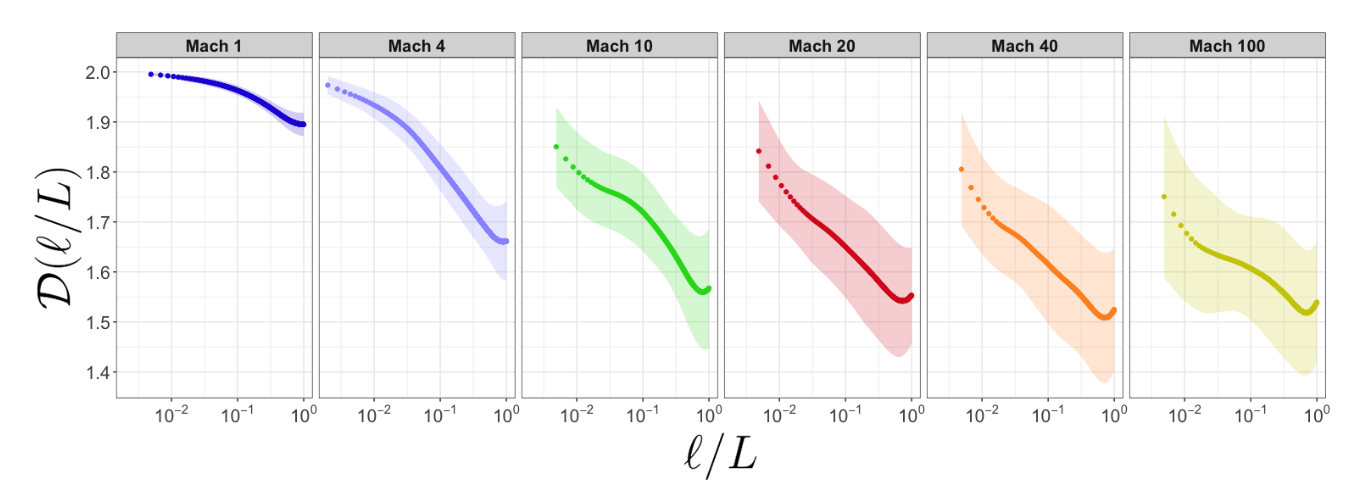
\includegraphics[width=0.85\textwidth]{figures/beattie_fractal_dimension.png}
    \caption{Fractal dimension derived from the mass–size relation as a function of Mach number \cite{beattie2019relation}.  
    Note that the x-axis is inverted relative to the representation used in our plots above.}
    \label{fig:beattie_fractal_dimension}
\end{figure}

As with the global method, certain limitations must be considered.  
Straight edges introduced by limited angular resolution at low column densities, as well as very small structures at the highest column densities, can affect the measurements.  
For these reasons, the usable column‑density range is narrower than the full range provided by the maps.

% Integrate topological insights (Euler characteristic).
Furthermore, the Euler characteristic highlights clear differences between Orion~A and Orion~B.  
Orion~A exhibits a profile that closely resembles the behavior expected from Gaussian Random Field simulations, with a well-defined peak at approximately \(1.64 \times 10^{22}\,\mathrm{cm}^{-2}\). For comparison, the results for a GRF are included in the Appendix in Figure \ref{fig:sims_euler_char}. 
This threshold is significant, echoing the transition seen in the global fractal dimension analysis, and marks the emergence of dense cores within the cloud.

In contrast, Orion~B shows no such pronounced peak, instead displaying a more gradual, almost linear decrease.  
If Orion~B is indeed more strongly influenced by turbulence, this behavior is consistent with a more scale-free, less clustered structure, where the appearance of dense cores is more gradual and widely distributed.  
The topological analysis therefore reinforces the notion that turbulence governs the structural evolution of Orion~B, while Orion~A undergoes distinct transitions closely tied to star-formation thresholds.

% explain visually some more also connected to the stuff above
Visual examples of the changes in the Euler characteristic for Orion~A and Orion~B are provided in Figures~\ref{fig:Euler_Orion_A} and~\ref{fig:Euler_Orion_B}.  
These figures illustrate how the degree of connectivity and fragmentation evolves as a function of column density.  

In Orion~A, the sharp peak in the Euler characteristic corresponds to a rapid transition from a regime dominated by isolated structures to one in which these structures merge into a more interconnected network.  
The example cutouts in Figure~\ref{fig:Euler_Orion_A} highlight this process: at low column densities, the cloud consists of one big connected structure surrounded by many disconnected regions; at mid range that starts to change, whereas at higher thresholds these regions coalesce into larger, more complex entities.
This marks the transition from a regime of many disconnected structures to one where connectivity increases rapidly.

In contrast, Figure~\ref{fig:Euler_Orion_B} for Orion~B shows a more gradual evolution.  
Here, the Euler characteristic decreases smoothly, indicating that fragmentation and merging occur over a broader range of column densities.  
The visual examples confirm that Orion~B maintains a predominantly filamentary and interconnected morphology across scales, consistent with its interpretation as a more turbulent, scale‑free environment.

For visualization, the column density threshold corresponding to the peak in the Euler characteristic for OrionA—along with the same threshold overlaid on OrionB for comparison—is shown in Figures~\ref{fig:gallery_euler_OA} and~\ref{fig:gallery_euler_OB} in the Gallery.
Together, these visualizations reinforce the quantitative findings and provide intuitive insight into how topology and morphology change across different physical regimes in the two clouds.

\begin{figure}[t]
    \centering
    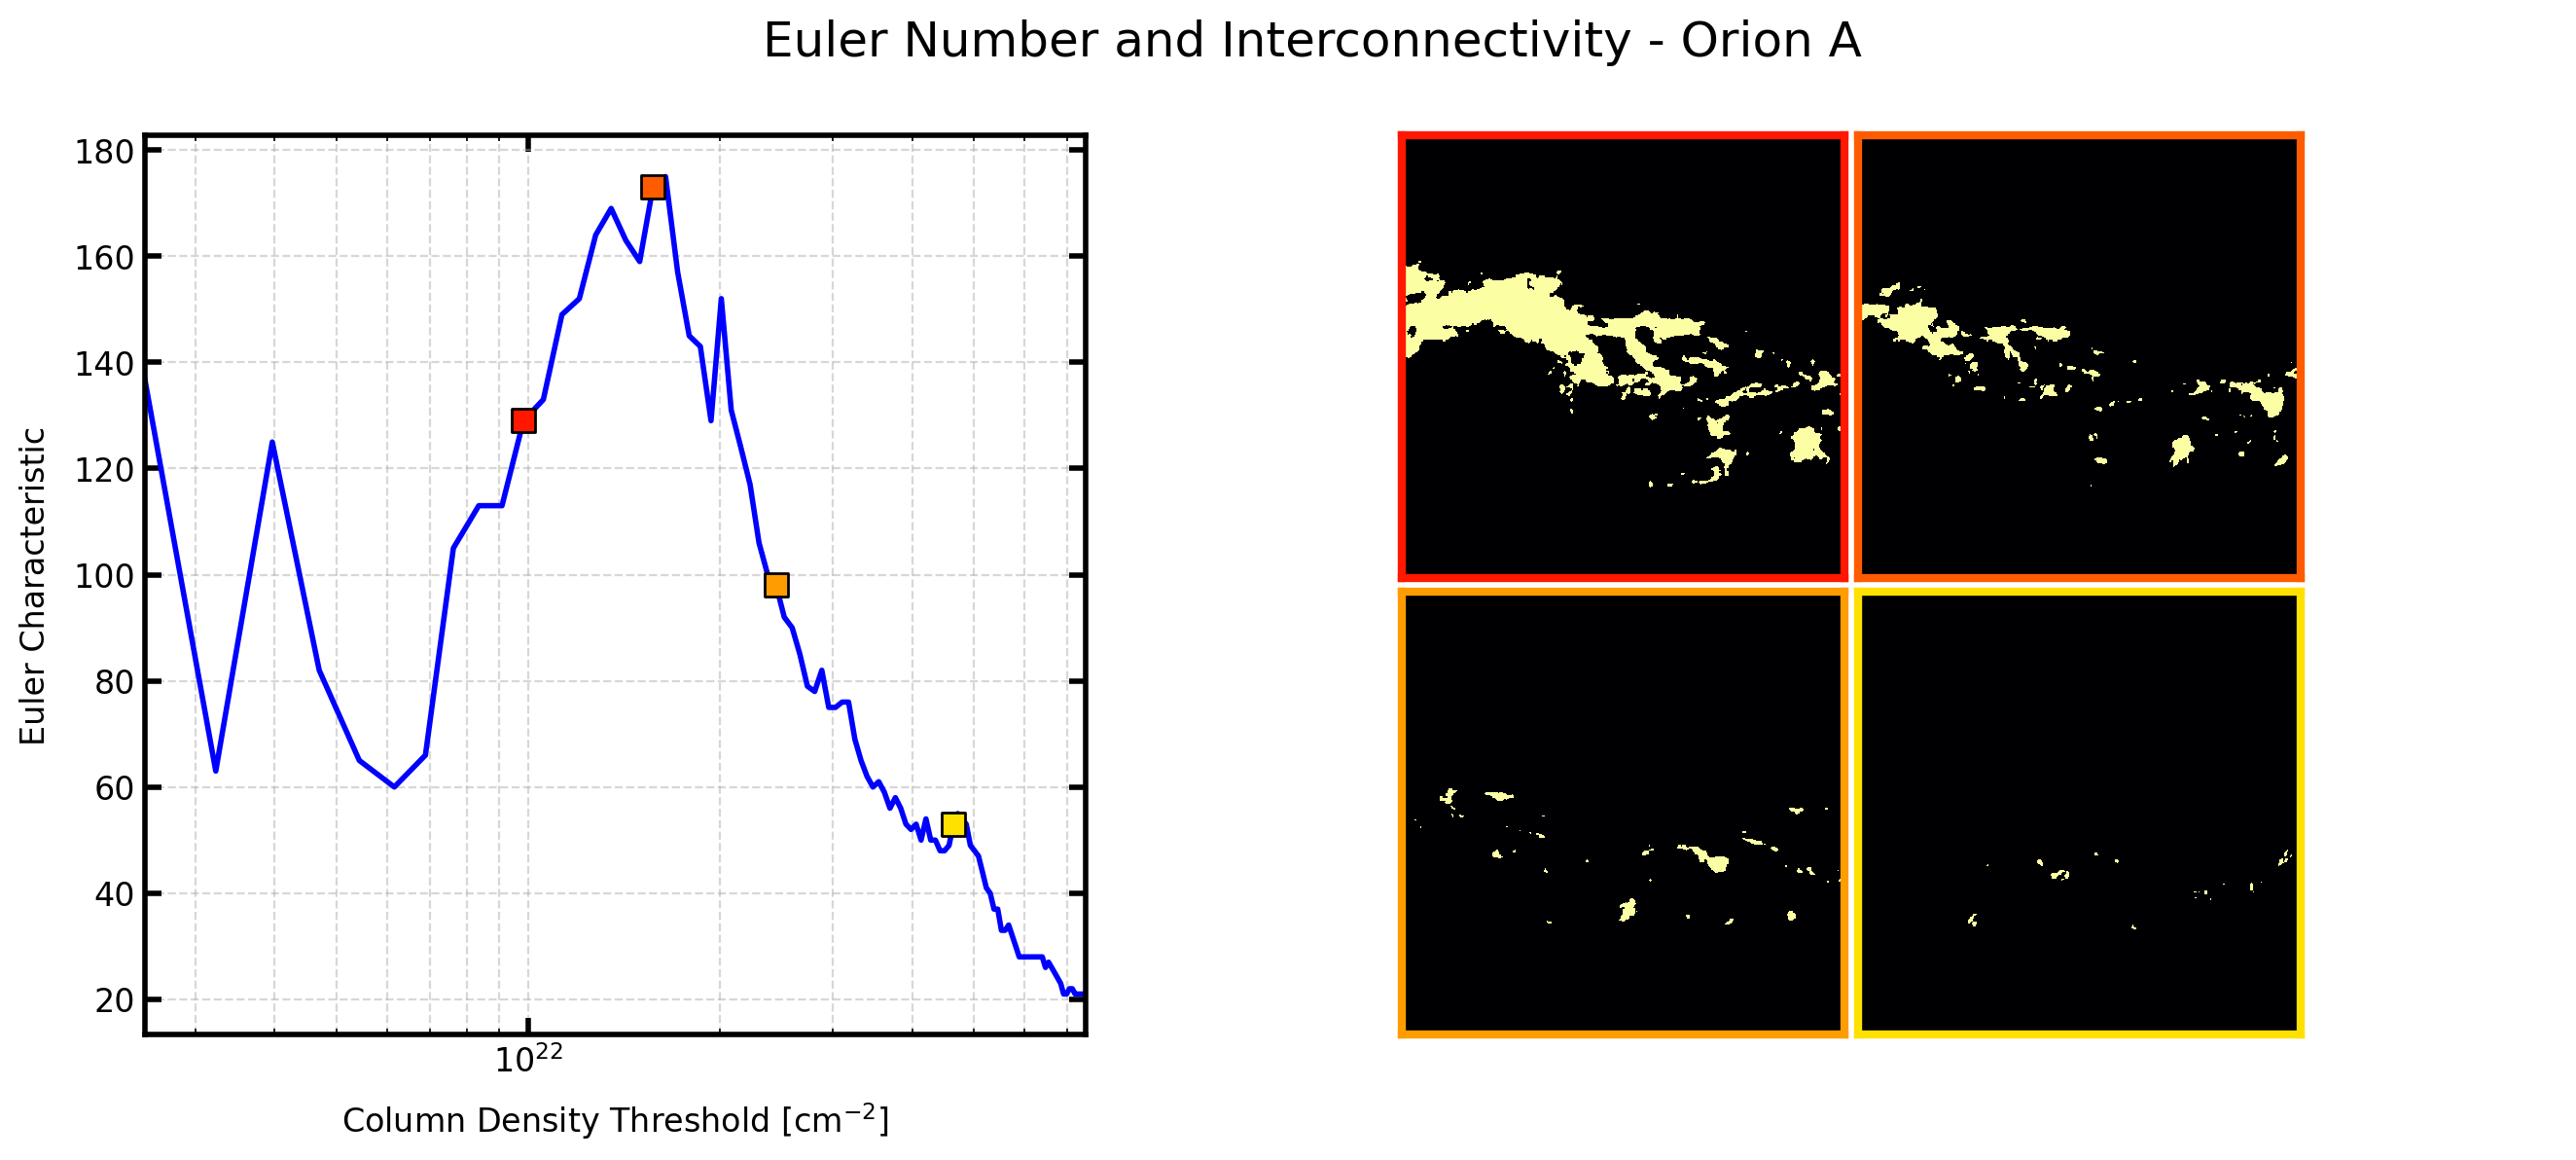
\includegraphics[width=0.85\textwidth]{figures/euler_Orion_A.png}
    \caption{Euler characteristic as a function of column density (left). The right panels show the same zoomed-in area of the cloud at the thresholds indicated by the colored boxes on the graph (Orion A).}
    \label{fig:Euler_Orion_A}
\end{figure}

\begin{figure}[t]
    \centering
    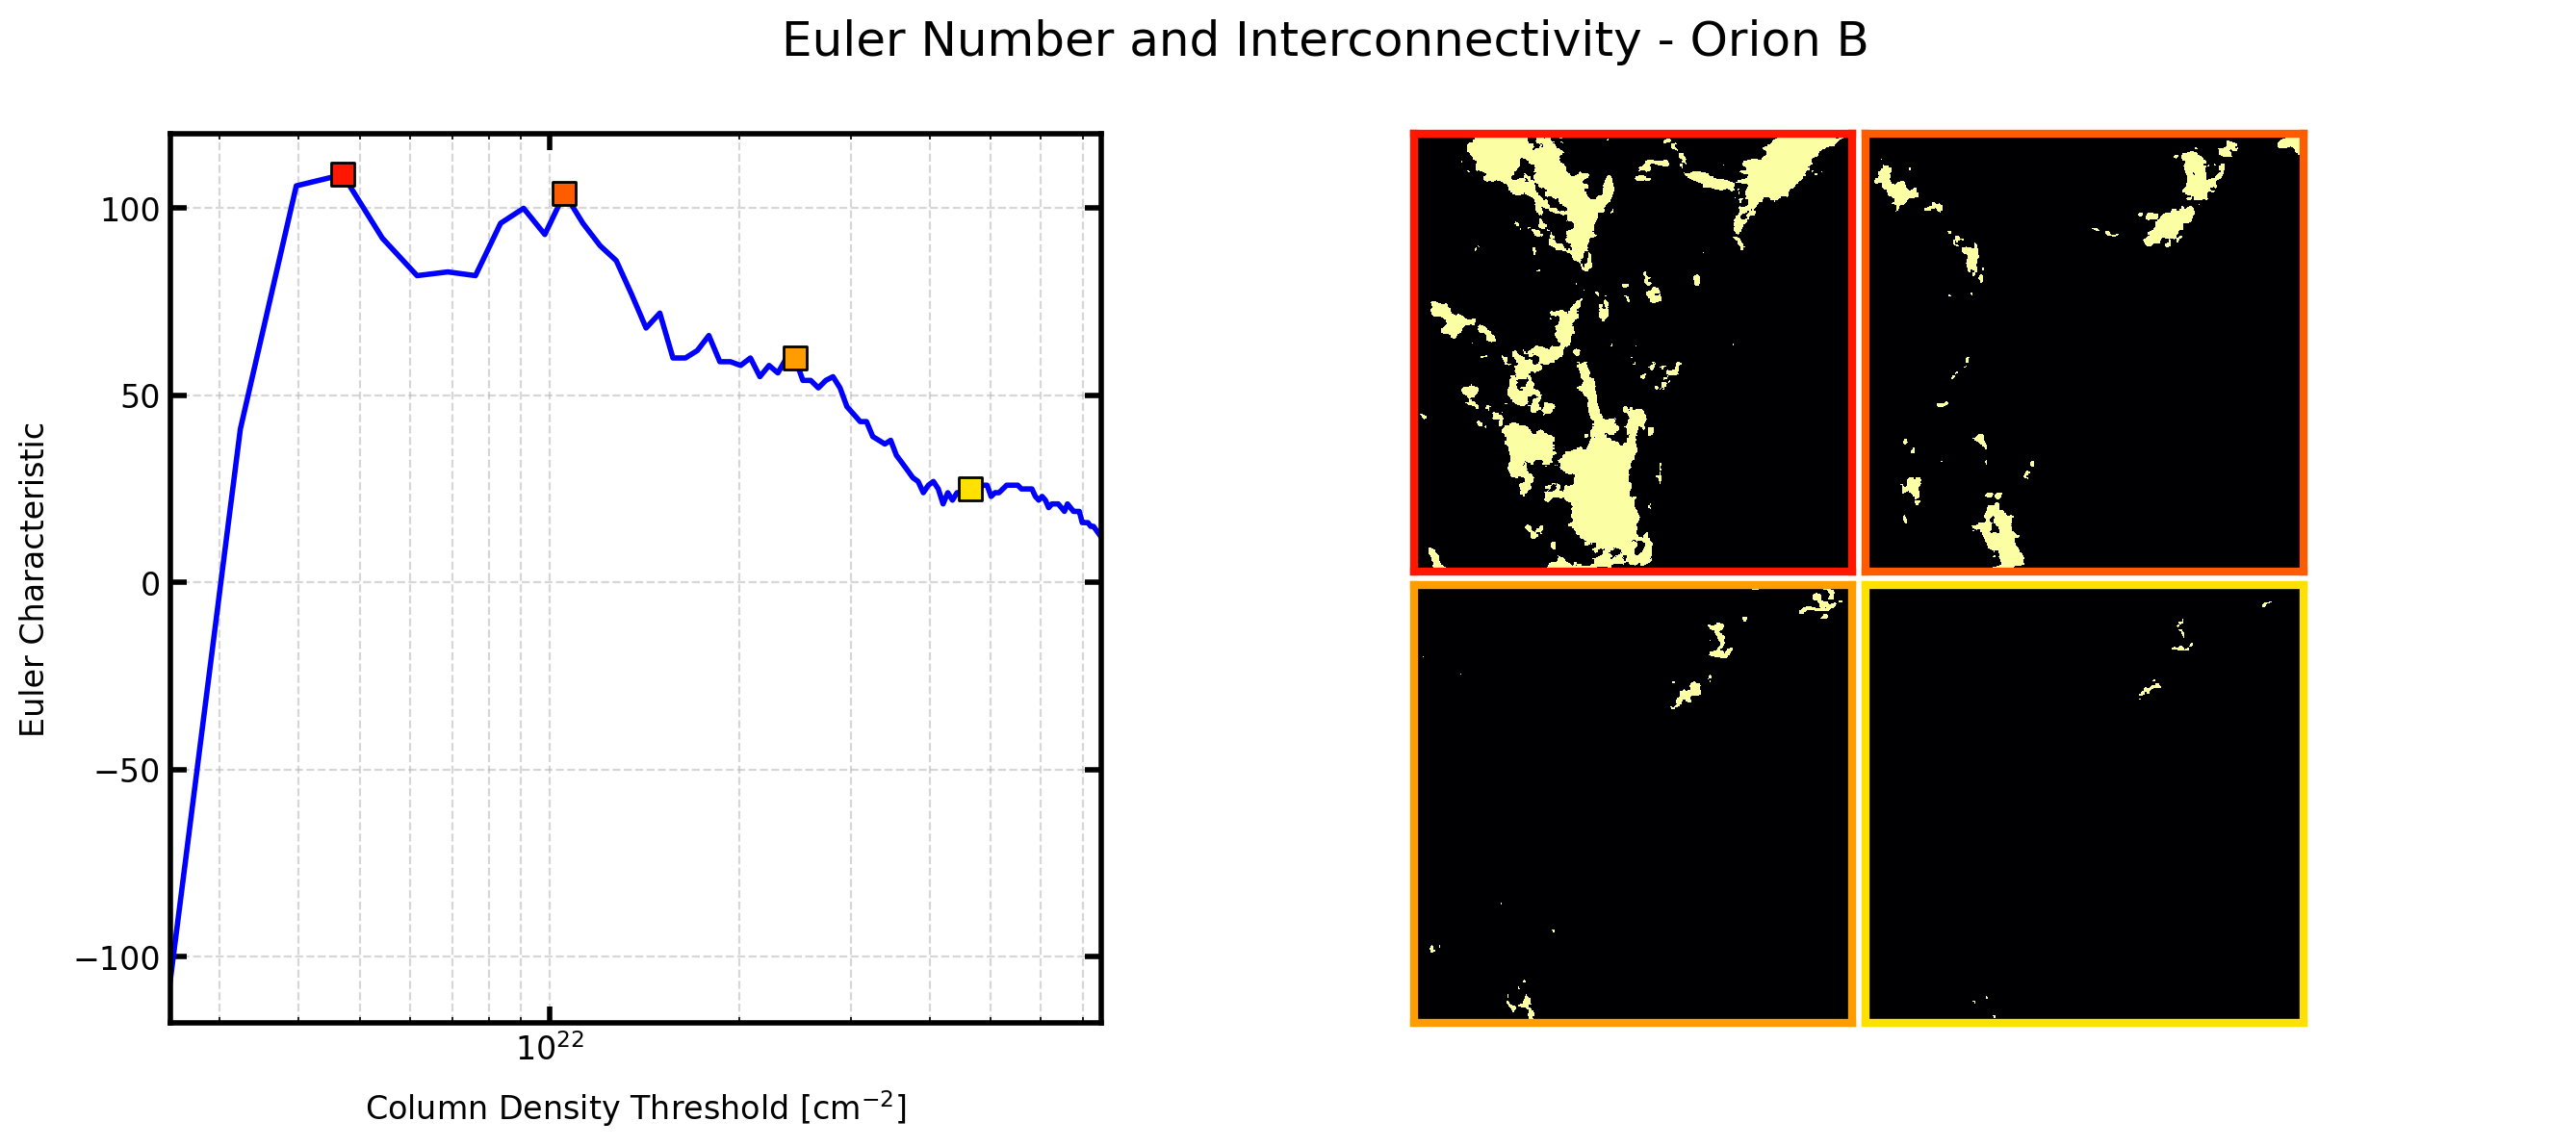
\includegraphics[width=0.85\textwidth]{figures/euler_Orion_B.png}
    \caption{Euler characteristic as a function of column density (left). The right panels show the same zoomed-in area of the cloud at the thresholds indicated by the colored boxes on the graph (Orion B).}
    \label{fig:Euler_Orion_B}
\end{figure}

% Bring in the MSD plane and individual-structure analysis.
% connect "hairy caterpillar" aspects
The next step in our analysis was to examine individual structures in the context of the local fractal dimension.  
Using the hierarchical segmentation provided by the dendrogram, we tracked the properties and positions of individual components at each column-density threshold.

As an initial step, we analyzed how the local fractal dimension of these structures varies with column density.  
We found that the ensemble of structures broadly follows the trend observed for the entire cloud, but with a shallower dependence and greater scatter (Figures~\ref{fig:local_A_single_structures} and~\ref{fig:local_B_single_structures}).  

These results raise interesting questions.  
While the ensemble as a whole tends toward \(D \approx 2\) (indicating increasing boundary complexity), one might expect that individual structures would appear smoother and simpler at higher column densities, rather than more intricate.  
This apparent tension motivates a closer look at how structure fragmentation and connectivity influence the derived fractal dimension.

Connecting the fractal dimension with mass and size properties further confirmed this puzzling picture: the smaller and lighther (core-like) the structures, the more they tend towards higher local fractal dimension (Figures \ref{fig:MSD_orion_A}, \ref{fig:MSD_orion_B}, \ref{fig:MSD_orion_A_B}).

The trends discussed in the MSD plane can also be verified visually using the gallery in Appendix~\ref{appendix:gallery}.
For OrionA, we begin with large-scale, low-fractal-dimension structures that encompass much of the cloud (see Figure\ref{fig:gallery_MSD_A_1}). These correspond to the upper-right region of the MSD plane, representing high mass and size but relatively low structural complexity.

As we move across the MSD diagram—decreasing in size and mass—the local fractal dimension tends to increase.
This progression is illustrated in Figures~\ref{fig:gallery_MSD_A_2}, \ref{fig:gallery_MSD_A_3}, and \ref{fig:gallery_MSD_A_4}, which show increasingly fragmented structures with more intricate boundaries.

At the extreme end, small and simple shapes dominate, often showing very high local fractal dimensions (approaching 2).
An example of such a structure is shown in Figure~\ref{fig:gallery_MSD_A_5}.
The mass, size, and fractal dimension of each example are shown in the figure labels to allow for direct comparison with the corresponding location on the MSD plane.

A similar pattern is observed in OrionB.
Figure\ref{fig:gallery_MSD_B_1} corresponds to the top right of the MSD plane—large, coherent structures with lower fractal dimension.
Figures~\ref{fig:gallery_MSD_B_2}, \ref{fig:gallery_MSD_B_3}, and \ref{fig:gallery_MSD_B_4} illustrate the gradual transition toward smaller, more fragmented features.
Finally, Figure~\ref{fig:gallery_MSD_B_5} shows a compact, high-density structure with a high local fractal dimension, representative of the lower-left region of the MSD plot.

% comparison with other methods
In light of these findings, it is instructive to compare our approach with more historically used methods for estimating fractal dimensions in molecular clouds.  
Classical analyses, such as those presented in \cite{elmegreen1996fractal}, often relied on a scale-counting relation of the form
\[
N(\lambda > L) \propto L^{-D},
\]
where \(N\) is the number of self‑similar structures larger than a given scale \(L\), and \(D\) is the inferred fractal dimension.  
While this method provides a useful first‑order characterization of cloud hierarchy, it is inherently limited to counting structures across scales and does not directly incorporate information about their shapes, perimeters, or connectivity.

By contrast, the perimeter–area approach used in this work captures not only the size distribution of structures but also the complexity of their boundaries and how that complexity evolves with column density.  
When combined with topological diagnostics such as the Euler characteristic and hierarchical segmentation via dendrograms, this method offers a more nuanced view of how morphology and topology change across different physical regimes.  
Rather than yielding a single, scale‑averaged fractal dimension, our approach reveals distinct regimes within the same cloud (e.g., Orion~A) and connects those regimes to physically meaningful transitions such as the emergence of dense cores and the onset of star formation.

In summary, while historical methods such as the \( N(\lambda > L) \) scaling have been invaluable in establishing the fractal nature of molecular clouds, the combined perimeter–area and topological analysis employed here provides a more detailed, physically interpretable framework that links structural complexity directly to the underlying star‑forming processes.

% Connect to star formation.
Finally, we decided to explore a possible connection between local structural complexity and star formation activity. To do this, we used the YSO catalogue from \cite{megeath2012catalogue}, extracting a sample of young stellar objects (YSOs) from which we computed a YSO density map. This density map was then correlated with our previously derived local fractal dimension maps (Figures~\ref{fig:local_A_map} and~\ref{fig:local_B_map}). We first analyzed only early-stage YSOs and then repeated the analysis for the full YSO sample for completeness and comparison.

The correlation results, expressed in terms of both Pearson and Spearman coefficients, revealed distinct trends for the Orion~A and Orion~B clouds. In Orion~A, we found a stronger correlation when using the early-stage YSO sample (Pearson: 0.434, Spearman: 0.429) compared to the full sample (Pearson: 0.286, Spearman: 0.393). In contrast, Orion~B showed the opposite behavior, with a weaker correlation for the early-stage sample (Pearson: 0.288, Spearman: 0.244) and a stronger correlation for the full sample (Pearson: 0.399, Spearman: 0.340).

These results hint at possible environmental differences between the two regions.  
In Orion~A, the stronger correlation for early-stage YSOs suggests that the emergence of complex, fragmented structures is closely tied to the onset of star formation.  
Conversely, the weaker or more distributed trend in Orion~B may reflect a more turbulent, less clustered environment where star formation proceeds in a less organized manner, less dependent on localized structural complexity.  
This interpretation is consistent with long-standing observational evidence: Orion~A hosts a significantly higher density of protostars and young stellar objects, including the Orion Nebula Cluster and the Integral Shaped Filament, and is overall far more active in star formation than Orion~B \cite{megeath2012catalogue}.  
The contrasting correlations therefore align naturally with the known difference in star-forming activity between the two regions.

It is important to note, however, that the method is currently limited by the relatively small number of YSOs in the early-stage catalogue and the restricted spatial coverage of the YSO density maps. These limitations make it difficult to draw firm conclusions. Nevertheless, if future studies with larger and more complete datasets confirm these patterns, they would provide valuable evidence for fundamental differences in the star formation environments of Orion~A and Orion~B, and demonstrate the potential of fractal and topological analyses to shed light on the physical conditions governing star formation in molecular clouds.

% End with a synthesis.
% review
Taken together, our analysis provides a cohesive view of the structural and physical differences between Orion~A and Orion~B.  
The combination of global and local fractal dimension measurements, topological diagnostics through the Euler characteristic, and the hierarchical insights from the MSD analysis reveals that both clouds exhibit scale‑dependent behavior, but in distinct ways.  
Orion~A shows clear structural transitions—evident in the change of slope in the global perimeter–area relation and the sharp features in the Euler characteristic—marking the emergence of dense cores and a close connection between increasing morphological complexity and active star formation.  
In contrast, Orion~B maintains a more uniform, filamentary character and exhibits weaker correlations with local complexity, consistent with a more turbulent, scale‑free environment where star formation proceeds in a more distributed manner.  

The accuracy of the derived morphological properties, including the fractal dimension and Euler characteristic, is inherently limited by the resolution of the observational data. At high column density thresholds, the number of pixels above the cut becomes increasingly sparse, which can lead to artificial fluctuations in the measured quantities—particularly in small or isolated structures. This effect may manifest as spurious peaks or enhanced scatter in the local fractal dimension. Conversely, at low column densities, smoothing and beam convolution can oversimplify the intrinsic cloud structure, potentially underestimating its complexity. While efforts were made to exclude clearly unphysical cases (e.g., regions with too few pixels or straight-edged artifacts), care must be taken in interpreting trends near the resolution limits. 
Future observations at higher angular resolution could help better resolve small-scale features and test the robustness of the patterns observed here.

These findings reinforce the idea that turbulence and self‑similarity dominate cloud structure on large scales, but that localized physical processes such as core formation can imprint strong deviations from scale‑free behavior.  
By integrating fractal analysis with topological measures and comparisons to simulations, this study demonstrates how a multi‑faceted approach can link the morphology of molecular clouds directly to their star‑forming activity, offering a richer and more physically grounded picture than classical methods alone.

% add discussion "hairy caterpillar" 
